\appendix  

\section{Pavyzdinis tiekimo grandinės modelis (Vertikalus)}
\begin{figure}[H]
    \centering
    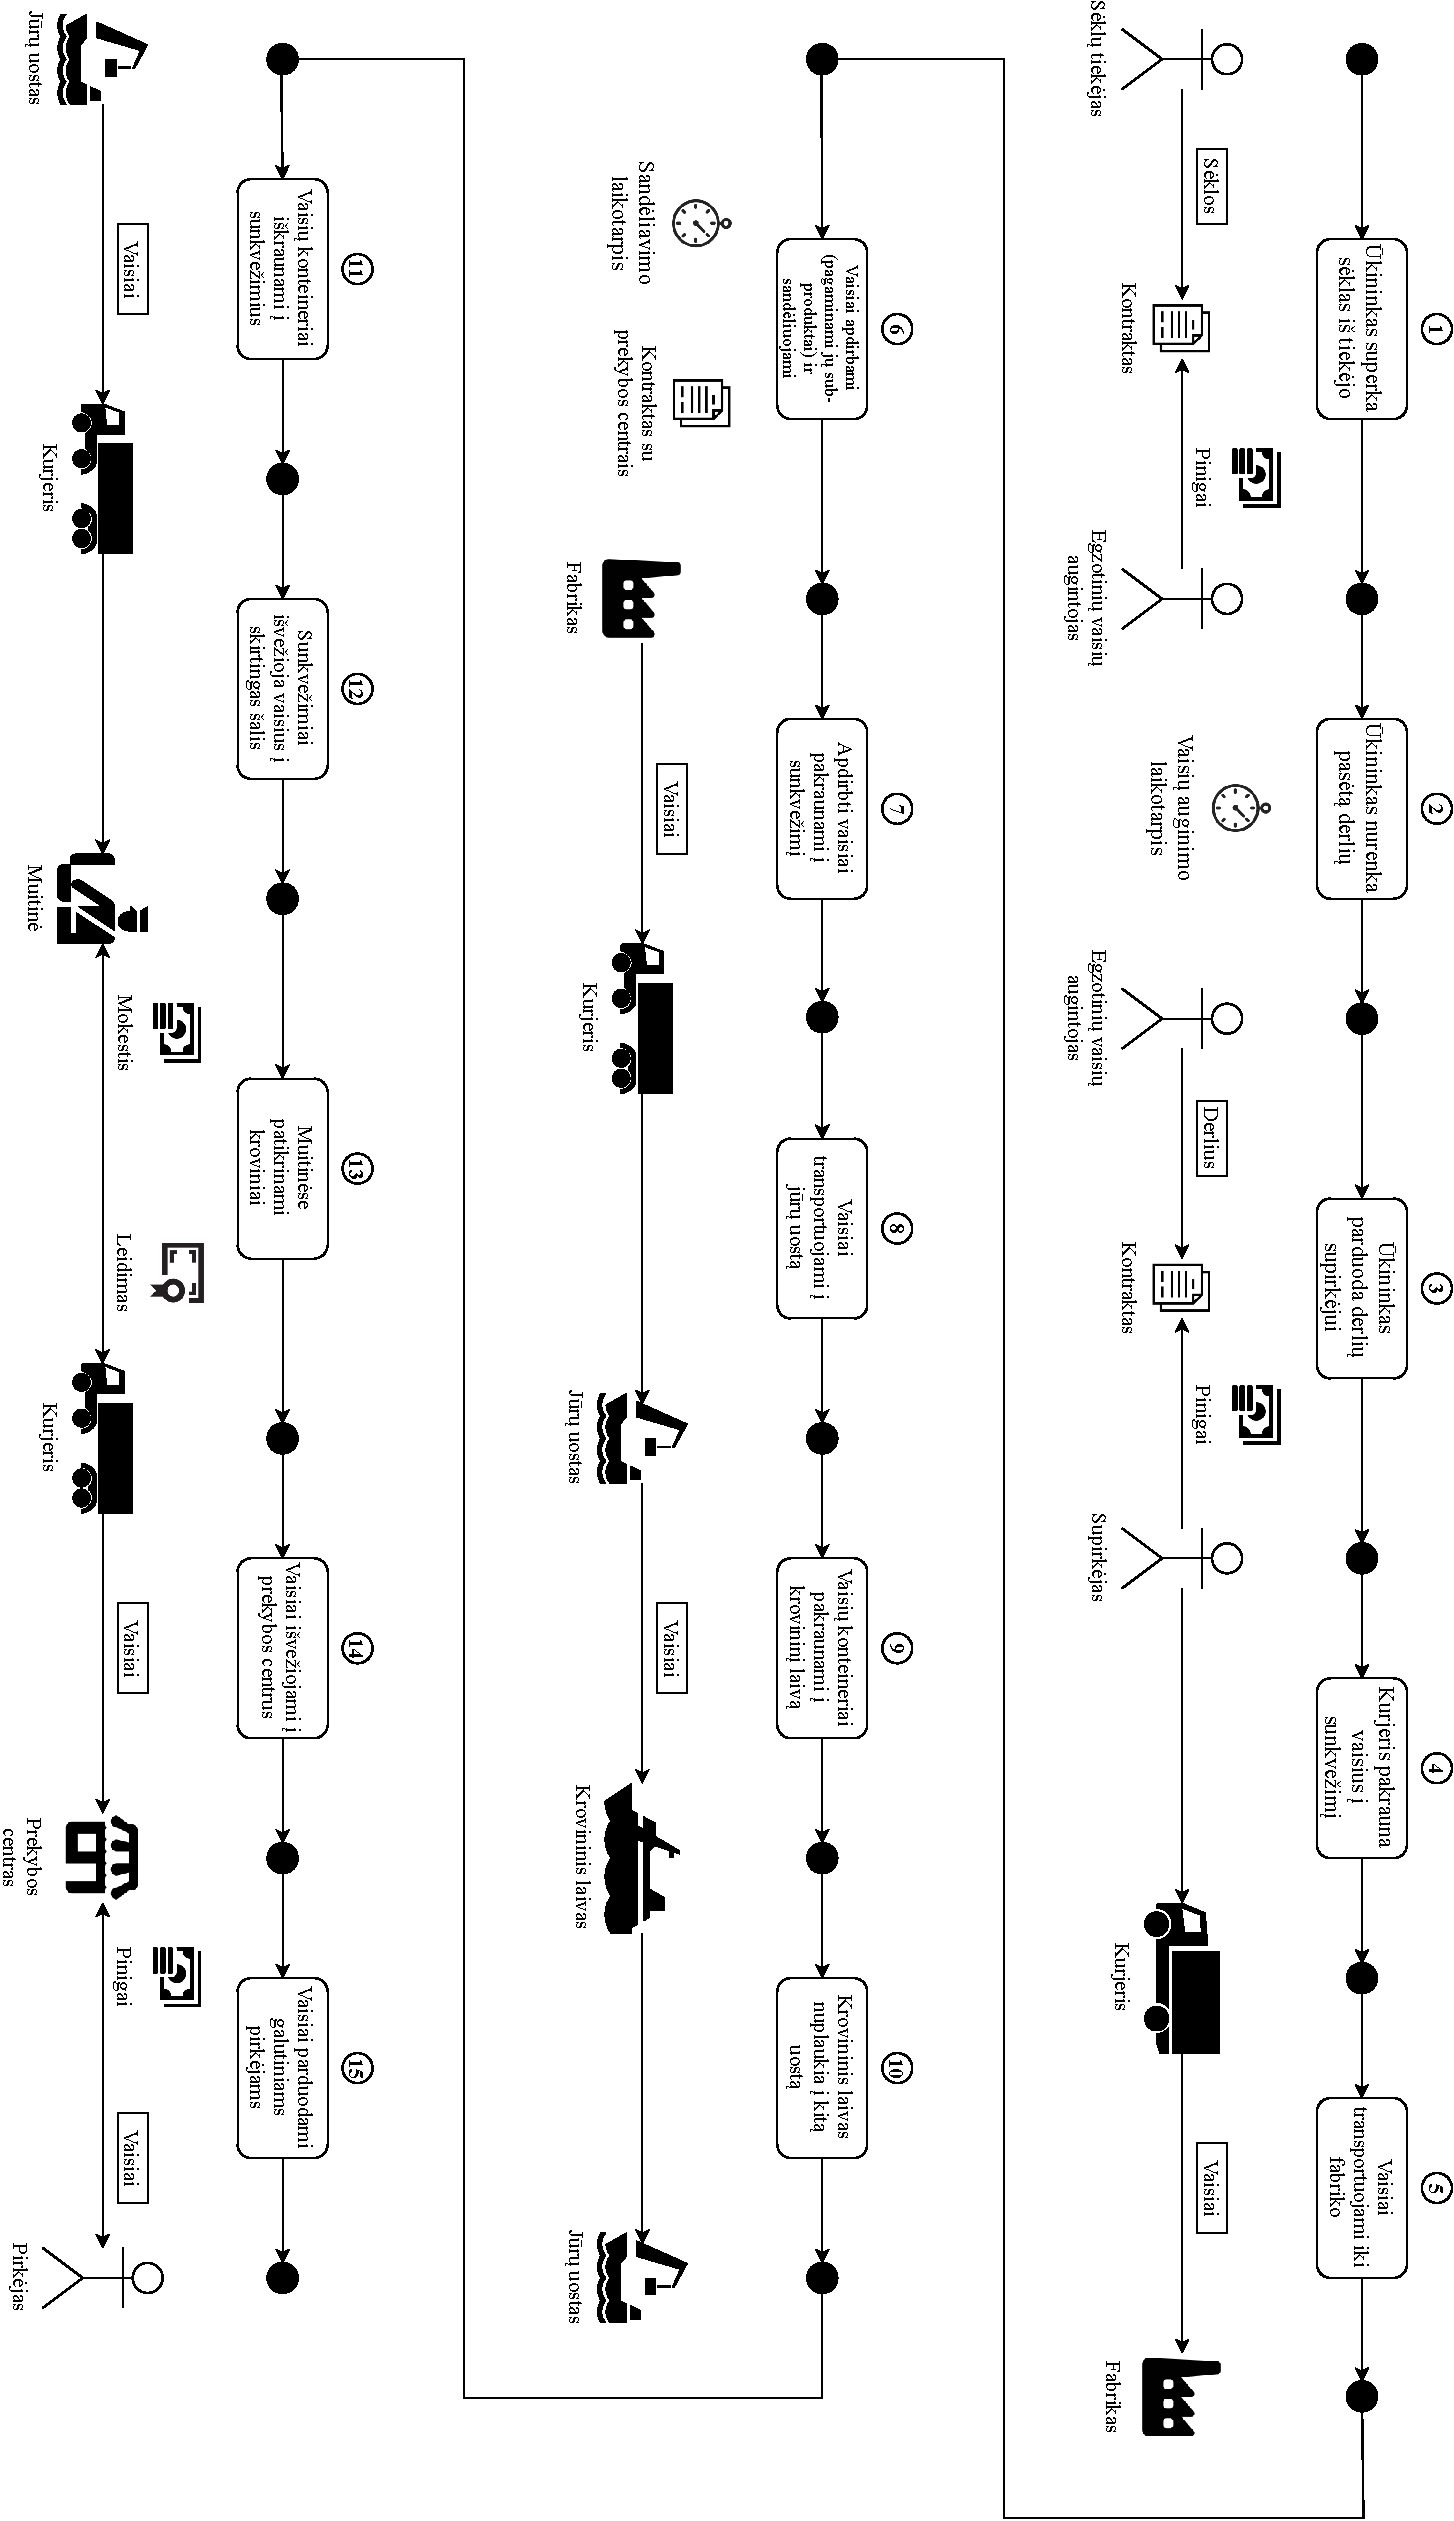
\includegraphics[scale=0.51]{images/supply-chain-vertical}
    \caption{Pavyzdinis tiekimo grandinės modelis (Vertikalus)}
\end{figure}



\section{Maskuotųjų nustatytos tapatybės pranešimų kanalo kūrimo ir prenumeravimo panaudos atvejai}
\begin{figure}[H]
    \centering
    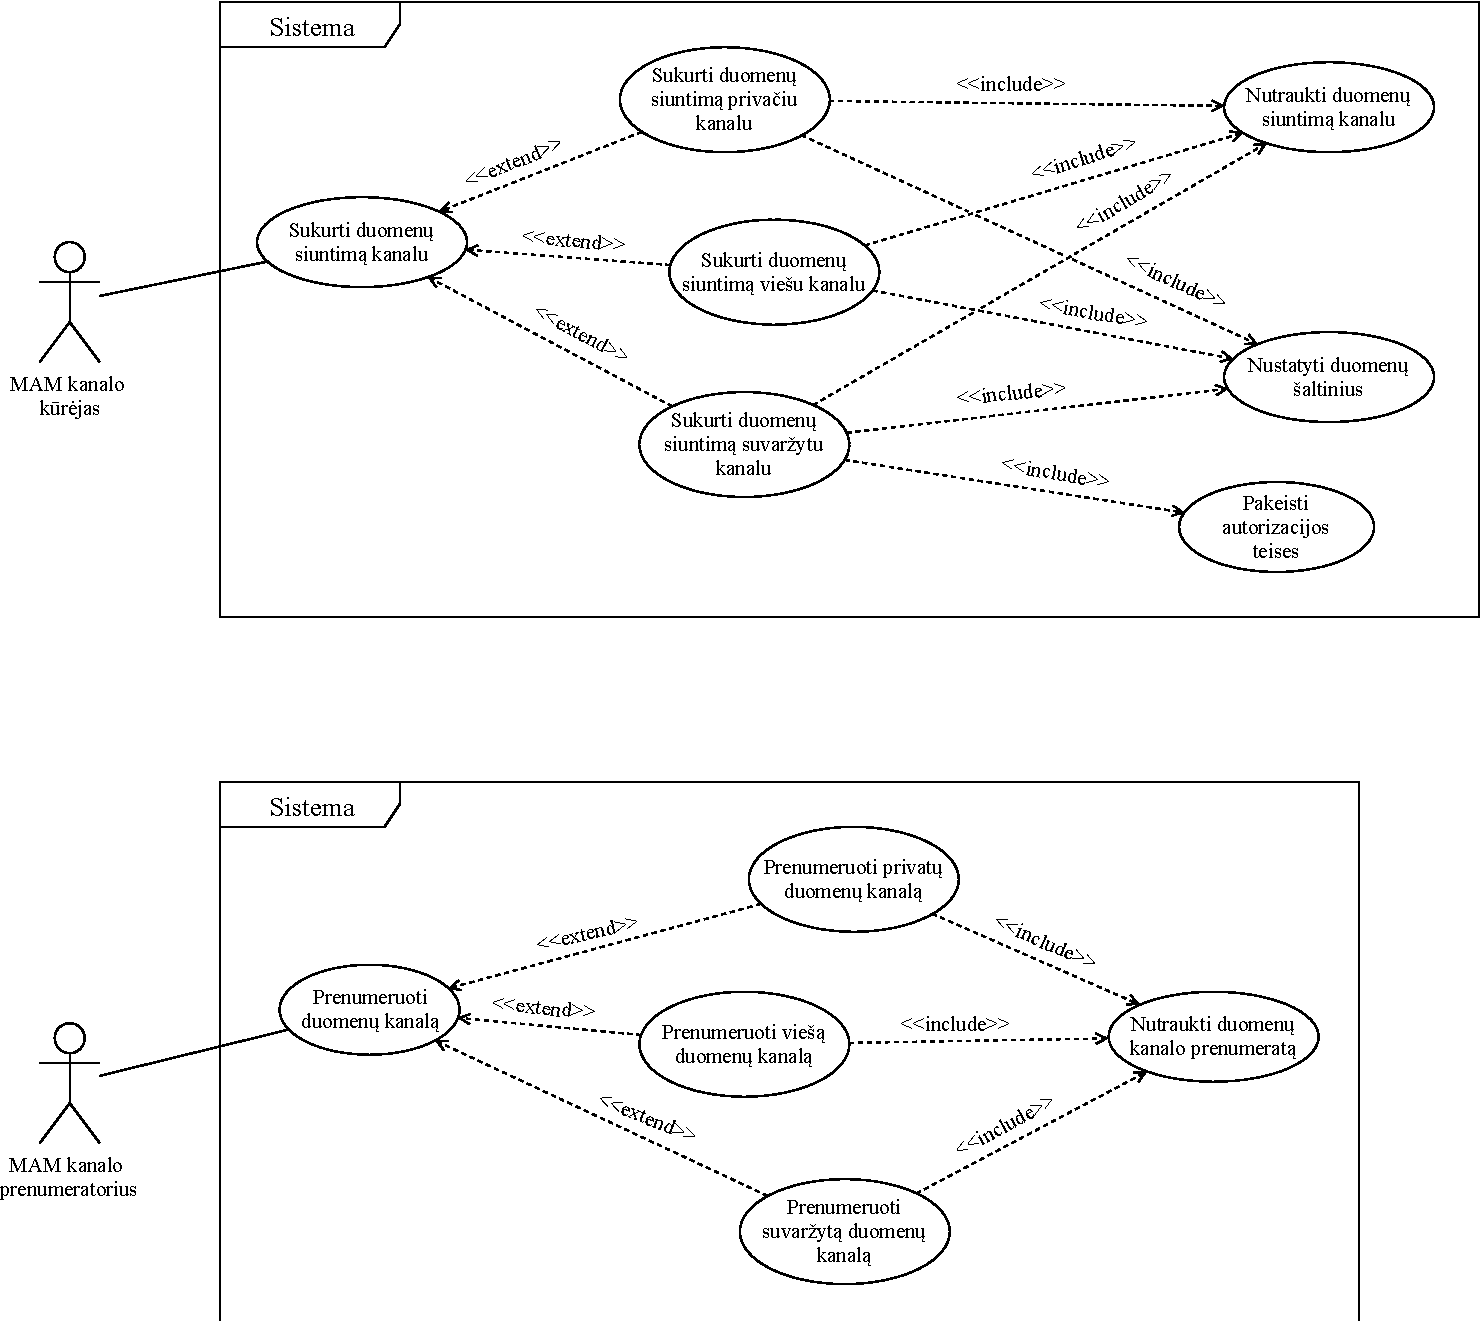
\includegraphics[scale=0.63]{images/ucd-1-2}
    \caption{MAM kanalo kūrimo ir prenumeravimo panaudos atvejai}
\end{figure}

\section{Kriptovaliutų pervedimo ir gavimo, QR kodo generavimo ir nuskaitymo bei sandorio kūrimo panaudos atvejai}
\begin{figure}[H]
    \centering
    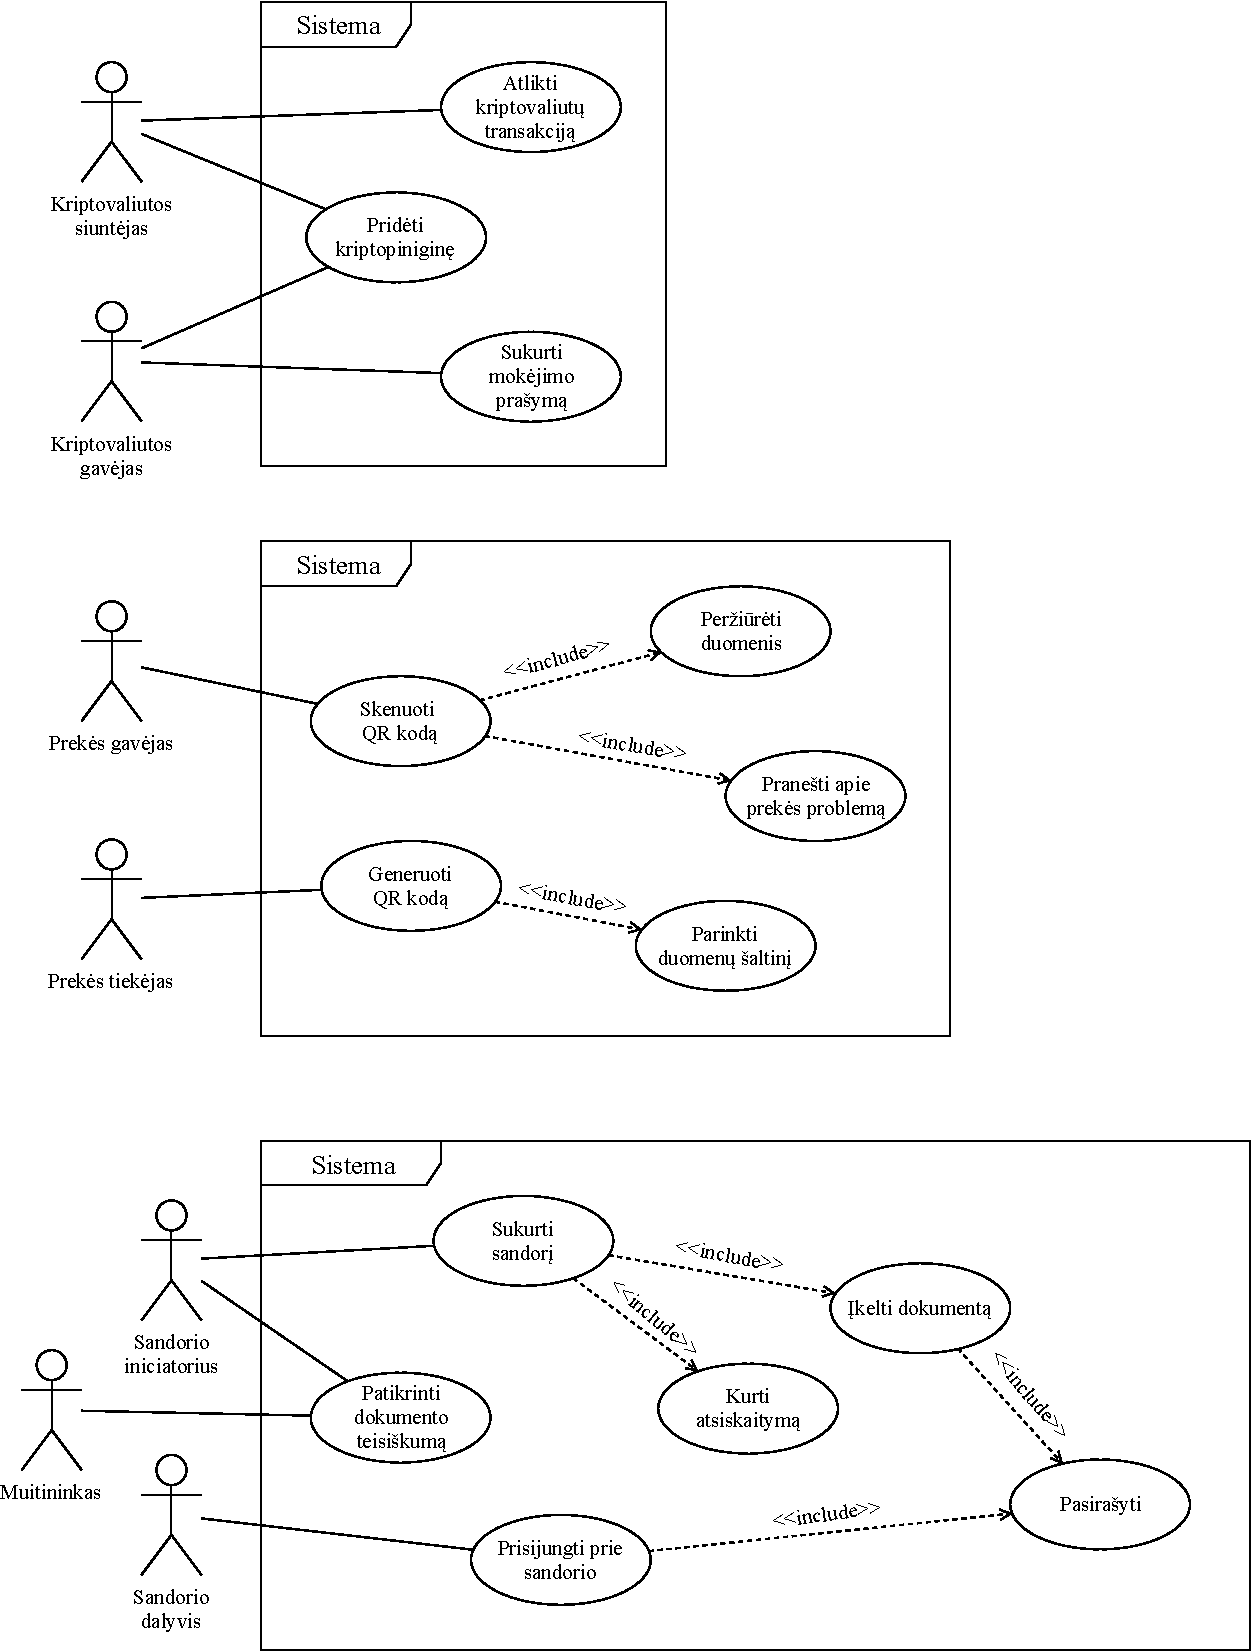
\includegraphics[scale=0.7]{images/ucd-3-4-5}
    \caption{Kriptovaliutų pervedimo ir gavimo, QR kodo generavimo ir nuskaitymo bei sandorio kūrimo panaudos atvejai}
\end{figure}



\section{Maskuotųjų nustatytos tapatybės pranešimų kanalo sukūrimo veiklų diagrama}
\begin{figure}[H]
    \centering
    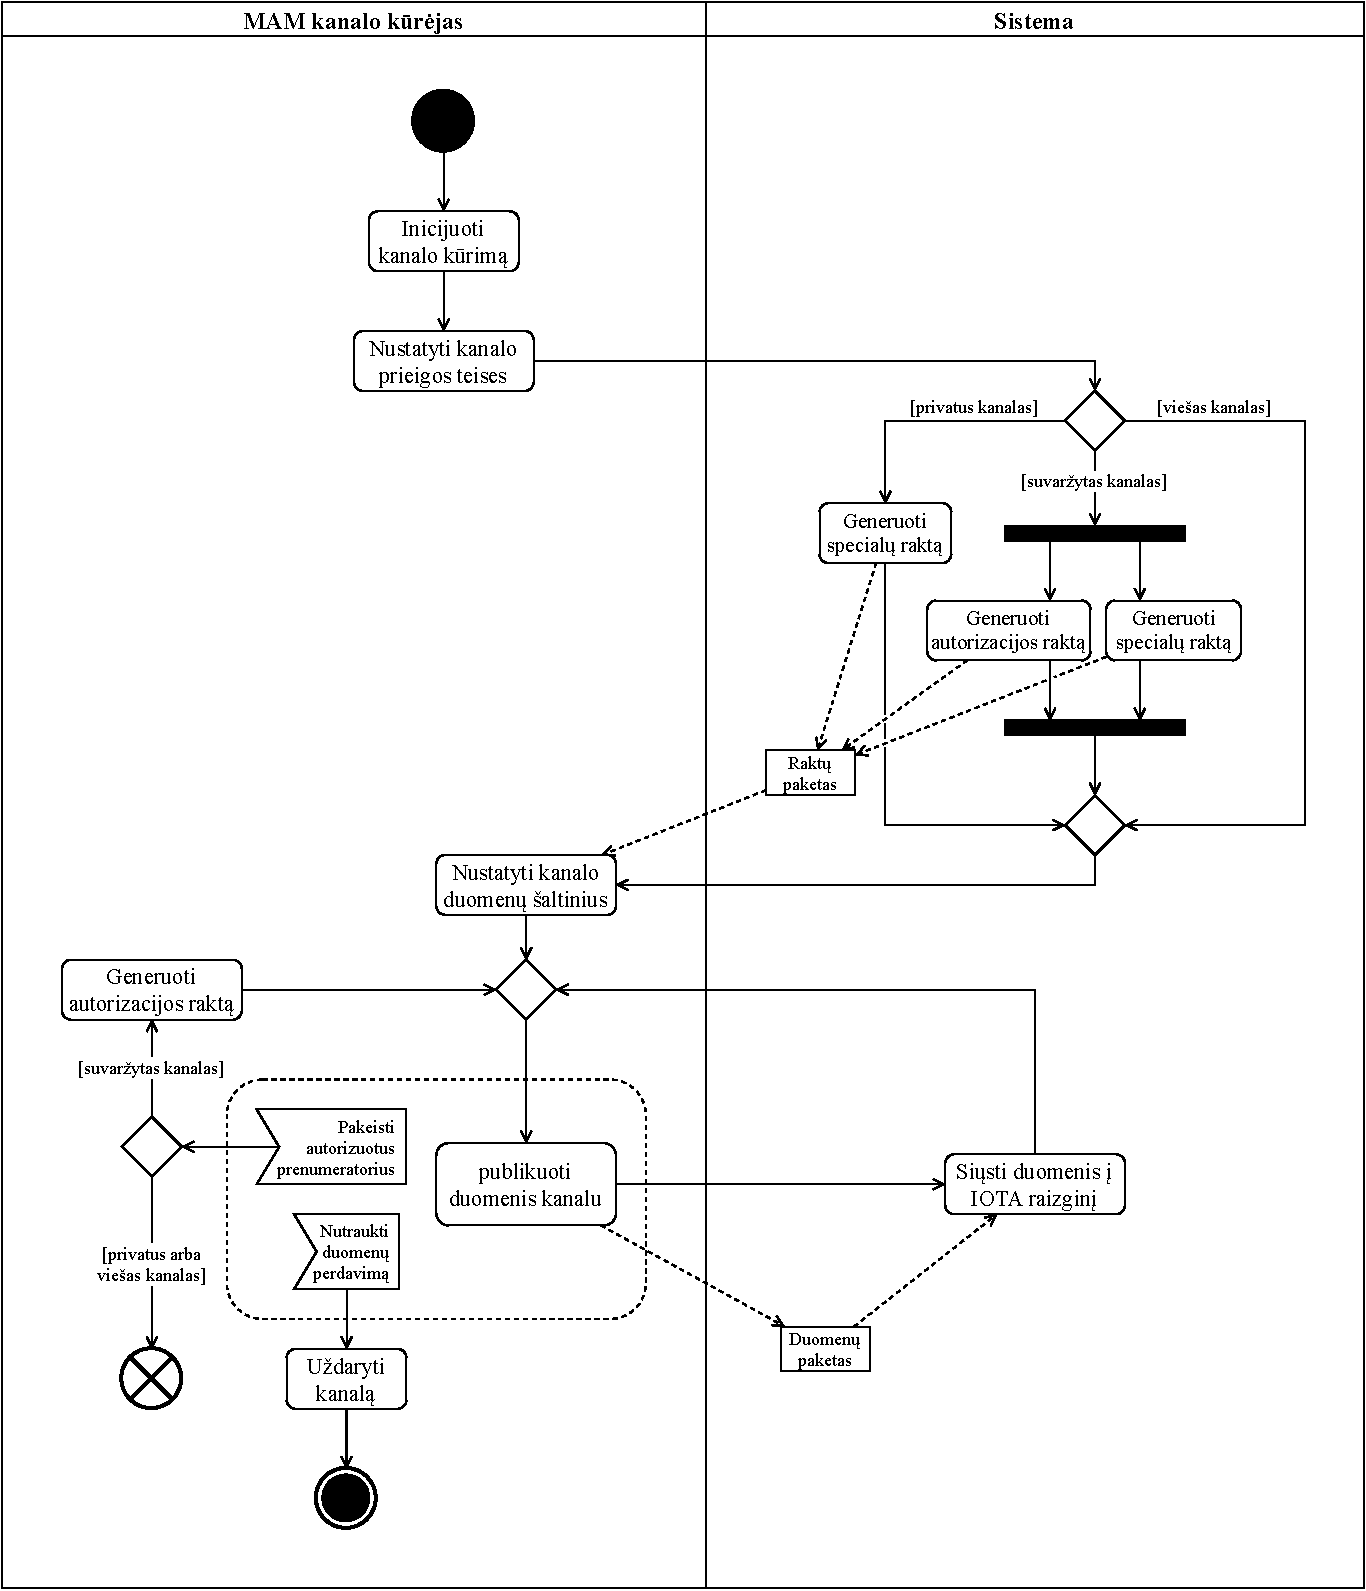
\includegraphics[scale=0.7]{images/ad-1}
    \caption{MAM kanalo sukūrimo veiklų diagrama}
\end{figure}

\section{Maskuotųjų nustatytos tapatybės pranešimų kanalo prenumeravimo veiklų diagrama}
\begin{figure}[H]
    \centering
    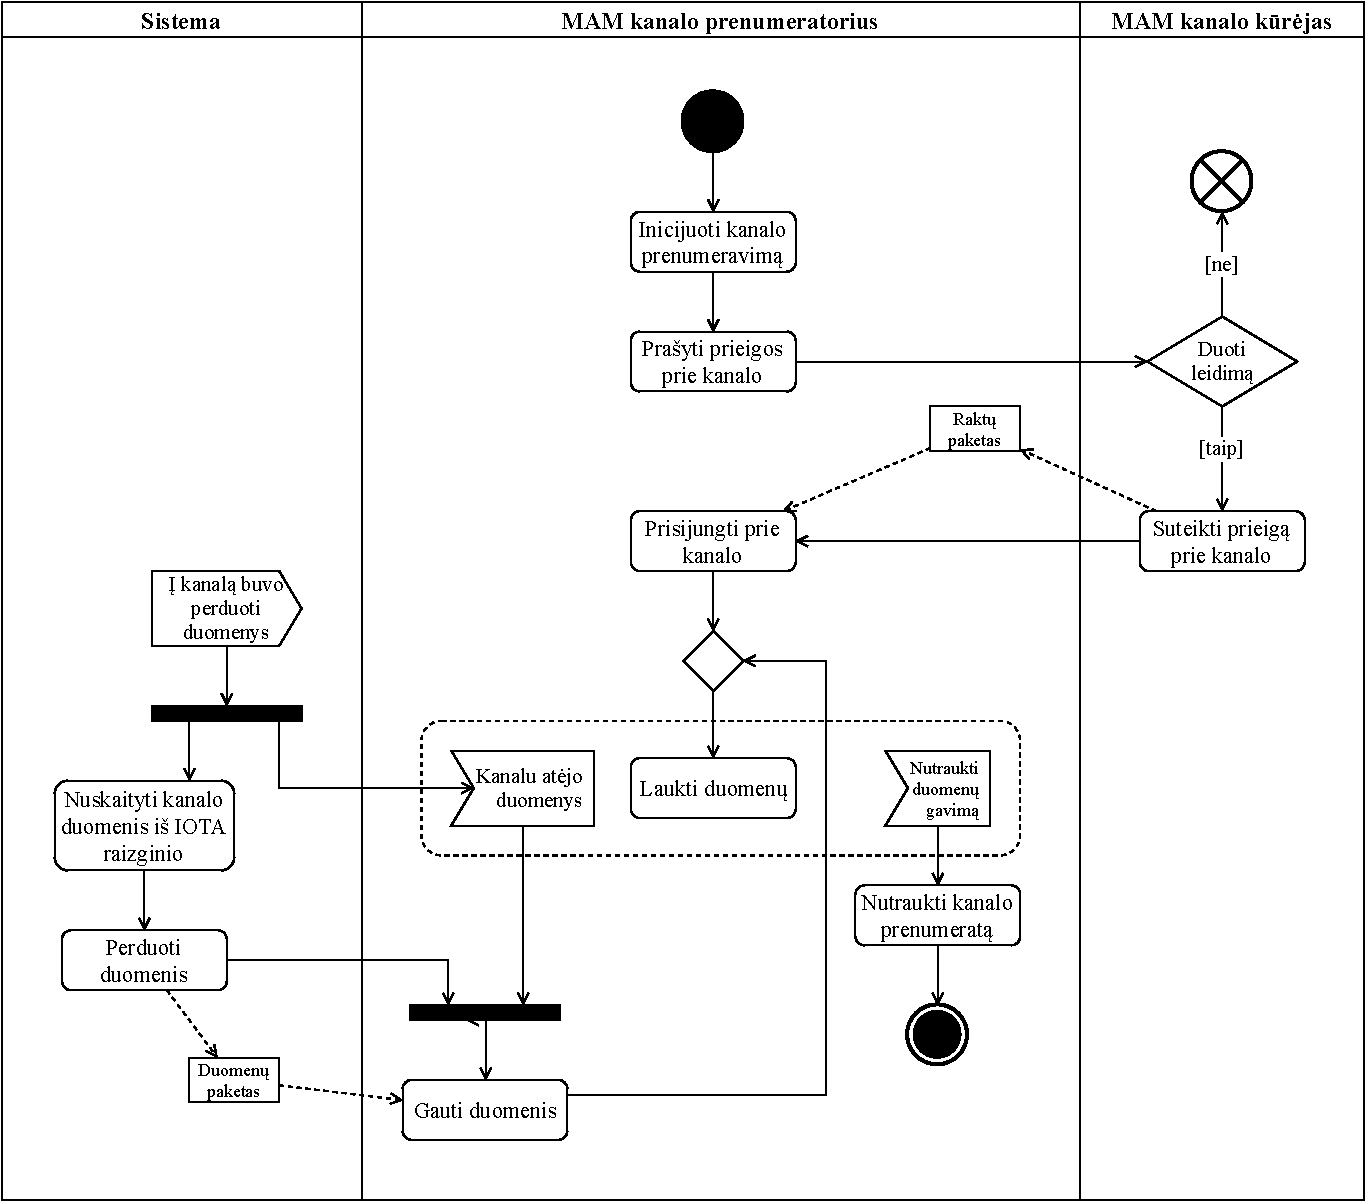
\includegraphics[scale=0.7]{images/ad-2}
    \caption{MAM kanalo prenumeravimo veiklų diagrama}
\end{figure}

\section{Kriptovaliutos siuntimo ir gavimo veiklų diagrama}
\begin{figure}[H]
    \centering
    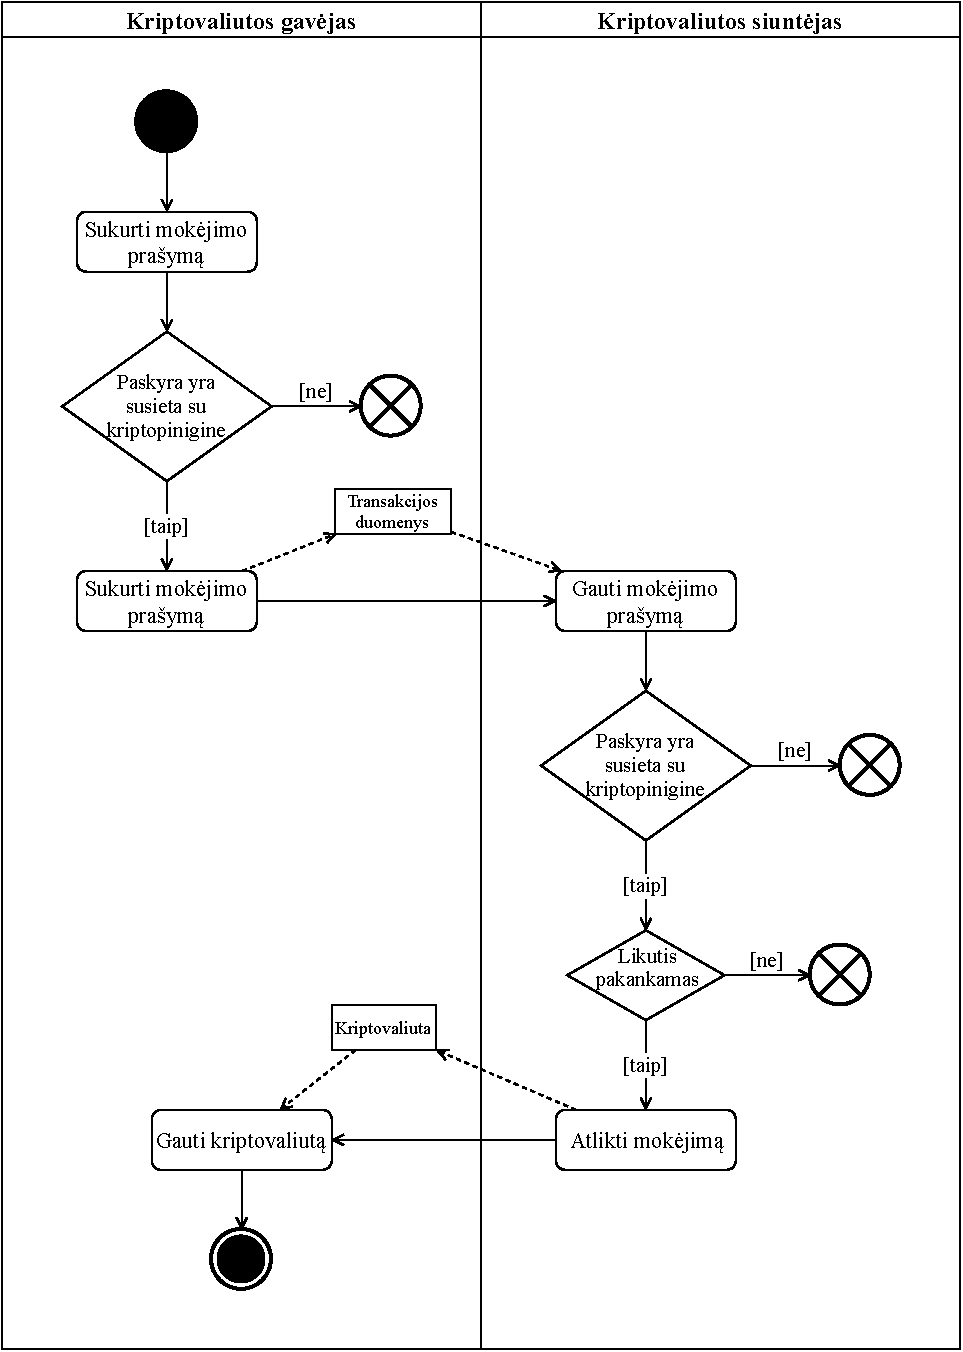
\includegraphics[scale=0.9]{images/ad-3}
    \caption{Kriptovaliutos siuntimo ir gavimo veiklų diagrama}
\end{figure}

\section{QR kodo generavimo ir nuskaitymo veiklų diagrama}
\begin{figure}[H]
    \centering
    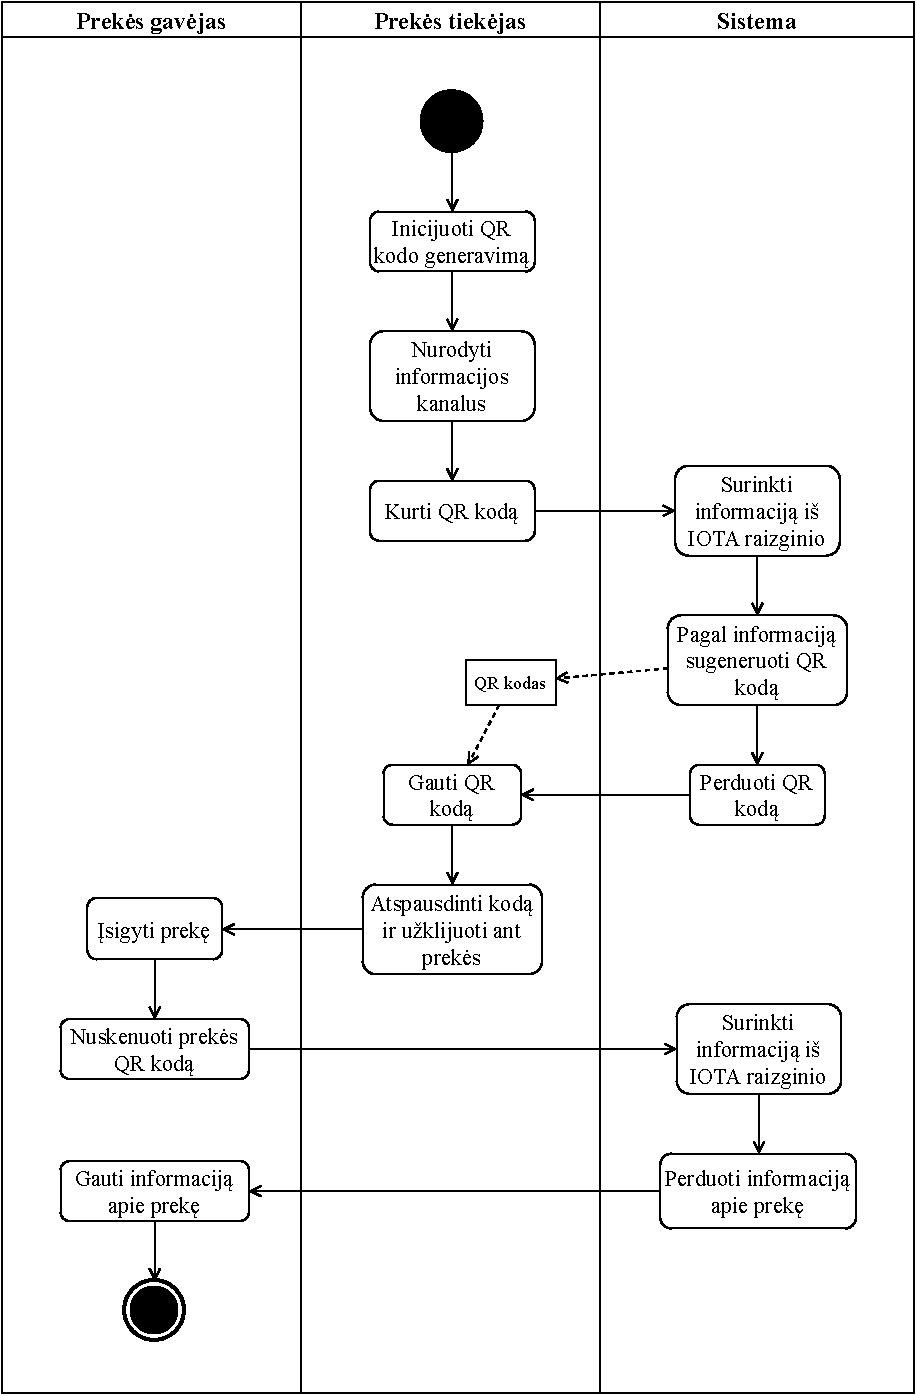
\includegraphics[scale=0.9]{images/ad-4}
    \caption{QR kodo generavimo ir nuskaitymo veiklų diagrama}
\end{figure}

\section{Sandorio sudarymo veiklų diagrama}
\begin{figure}[H]
    \centering
    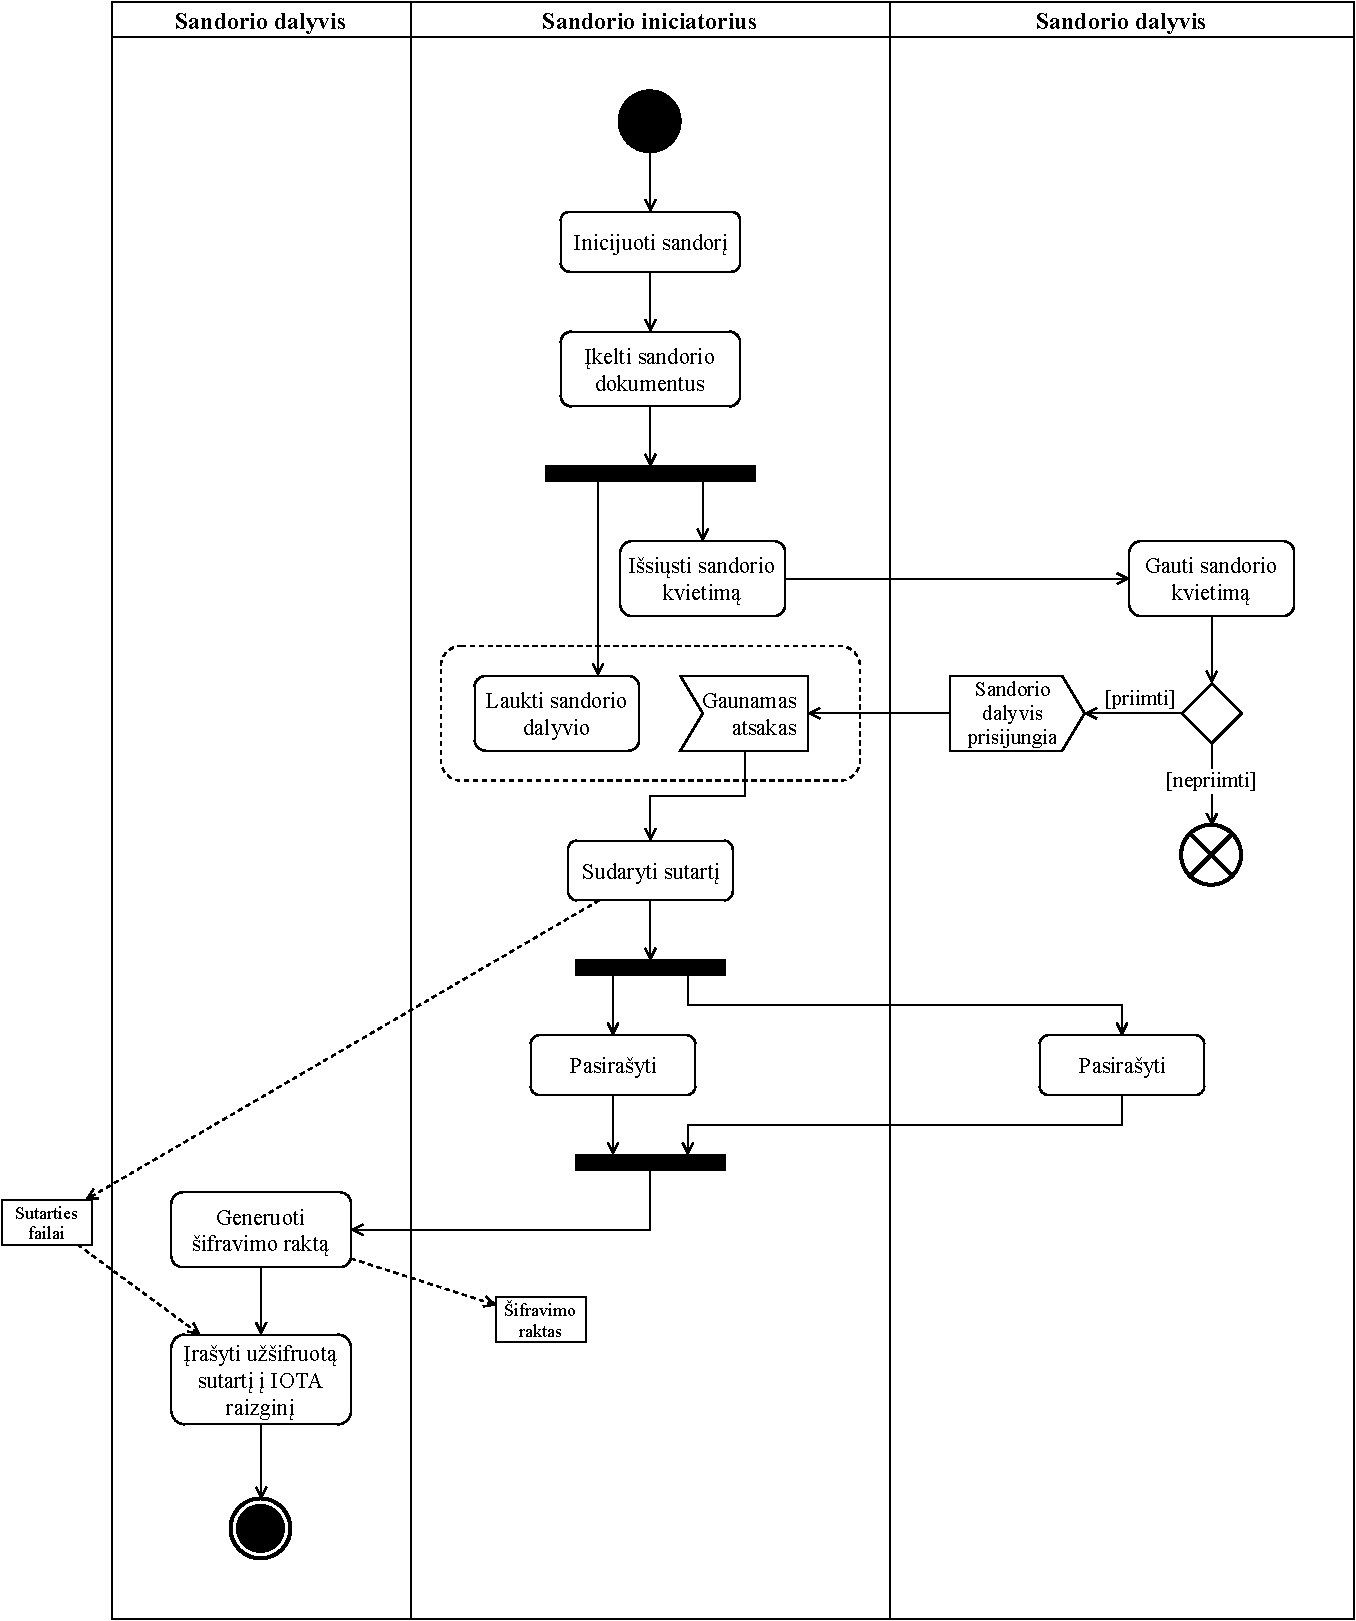
\includegraphics[scale=0.7]{images/ad-5}
    \caption{Sandorio sudarymo veiklų diagrama}
\end{figure}



% Prieduose gali būti pateikiama pagalbinė, ypač darbo autoriaus savarankiškai
% parengta, medžiaga. Savarankiški priedai gali būti pateikiami ir
% kompaktiniame diske. Priedai taip pat numeruojami ir vadinami. Darbo tekstas
% su priedais susiejamas nuorodomis.